\section{Semi-Markovian Model}
As it has been said before, the model applied in order to predict the behaviour of the primary system to take profit from the white spaces in the spectrum is the semi-markov model introduced in \cite{gts1}-\cite{gts3}. The main characteristic of the semi-markovian model is that allows an arbitrary specification of the holding time distribution in each state. Using a markovian model implies that the times distribution in each state must be exponentially distributed.

In Figure \ref{figure1spectrum} can be observed how the spectrum is composed of active and inactive (or idle) periods of communication. This idle periods are the called white space in which we want to focus on.

\begin{figure}[H]
\centering
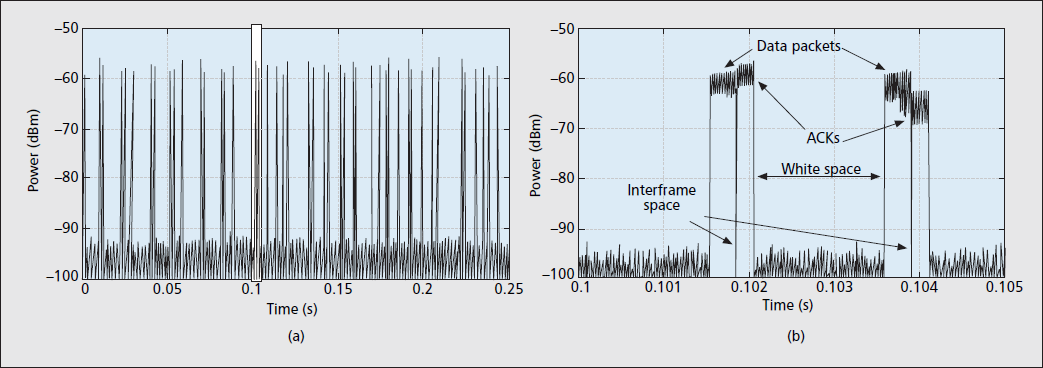
\includegraphics[width=\linewidth]{images/spectrum}
\caption{(a) Complex baseband signal of an 802.11b-WLAN supporting a Skype conference call; (b) enlarged view of two subsequent packet transmissions. \cite{gts4}}
\label{figure1spectrum}
\end{figure}

In \cite{gts1} different sensing methods are proposed to capture the traffic of the network. From the results of these captures, the channel can be classified in four different states. The channel can be busy because of the transmission of a data packet or an acknowledgement. On the other hand, the channel will be idle because of contention period of the stations or because there is no data to transmit. This leads to the following markov state scheme represented in Figure \ref{semi-markov}.

Additionally, the states Data, SIFS and ACK, can be considered as a single state ``Active'' which will give us the final two-state semi-markov process represented in Figure \ref{semi-markov}.

\begin{figure}[H]
\centering
\includegraphics[scale=0.5]{images/semi-markov}
\caption{Semi-Markov model}
\label{semi-markov}
\end{figure}

Considering that the states Data, SIFS and ACK correspond to the ``Active'' state and the states CW and WS corresponds to the ``Idle'' state, we can re-design our model to a two-state semi-markov scheme as is represented in Figure \ref{semi-markov2}.

\begin{figure}[H]
\centering
\includegraphics[scale=0.5]{images/semi-markov2}
\caption{Semi-Markov model simplification}
\label{semi-markov2}
\end{figure}

In \cite{gts1}, their measurement setup with high SNR and no hidden nodes, the three ``Active'' states represented in Figure \ref{semi-markov} are essentially deterministic (probability between states close to 1) if no collision is considered. From this, those three states can be considered as a single one.
On the other hand, this assumption cannot be extended also to the ``Idle'' states. As it is specified in \cite{gts1}, the different data rates give different behaviour:

\begin{flushright}
\small \textit{For small $\lambda$ we see heavy-tailed behavior, while for large $\lambda$ an exponential distribution seems to be a good fit.} [...] \textit{we focus on distributions whose shape can approximate both extremes. In particular, we consider a generalized Pareto distribution} [...]
\end{flushright}

However, in \cite{gts1} there is no differentiation in the behaviour of the CW and WS states. This is corrected in the following papers of the same autors \cite{gts2}, \cite{gts3}. In those documents, the model is extended considering a mixture of distribution to differentiate between the two states of the ``Idle'' period:

\begin{equation}
F(t;\theta)=p_cF_c(t)+(1-p_c)F_f(t;\theta)
\label{eq:idle_mixture}
\end{equation}

where $F_c(t)$ is the cdf of the contention window (considered uniform in [0,$T_c$]), $p_c$ the transition probability from WS to CW state and $F_f(t;\theta)$ denotes the generalized Pareto cdf of the unusued channel depending on the unknown parameter $\theta$.

From all these assumptions it is possible to simplify the model represented in Figure \ref{semi-markov} into the final model represented in Figure \ref{semi-markov2}. Its important to remind that their measurements and model definition are performed over a low traffic setup. Our intention in this project is to test if these assumptions can be also extended to high traffic schemes like the ones presented in \cite{hkps1}.